% !TeX root = ../main.tex

\section{Dynamic Model}
    \frame{\sectionpage}

    \begin{frame}
        \centering
        % \begin{equation*}
        %     V_{t}(x) = E\left[\max_{u \in \{0,1\}} \{R u + V_{t+1}(x- S u)\}\right]\end{equation*}
        % \end{equation*}
          \begin{equation*}
            V_{t}(x) = \sum_{i} \lambda_i \left[\max_{u \in \{0,1\}}\{s_i u + V_{t+1}(x- (1+s_i) u)\}  \right] + (1-\sum_i \lambda_i)V_{t+1}(x)
          \end{equation*}
             \begin{equation*}
               = \sum_{i} \lambda_i \left[\max\{s_i + V_{t+1}(x-1-s_i),V_{t+1}(x)\}\right] + (1-\sum_i \lambda_i)V_{t+1}(x)
             \end{equation*}
             \begin{equation*}
               = V_{t+1}(x) + \sum_{i} \lambda_i \left[\max\{s_i + V_{t+1}(x-1-s_i)-V_{t+1}(x),0\}\right]
             \end{equation*}
    \end{frame}

    \begin{frame}
      \begin{itemize}
        \item $x$, remaining capacity.
        \vspace{10pt}
        % \item $R,S$, random variable.
        % \vspace{10pt}
        \item $s_i$, the number of people $i$th type of group contains. If we suppose the number is continuous, then $s = \{1, \ldots,n\}$.
        \vspace{10pt}
        \item $\lambda_i$: the probability of an arrival of $s_i$.
        \vspace{10pt}
        \item $u$, binary variable. $u=1$, accept.
      \end{itemize}
    \end{frame}

    \begin{frame}{Properties of marginal value}
      \begin{itemize}
        \item $f(x) = \max_{a =\{0,1\}} \{a(p-1) +g(x-ap)\}$, $p = s_i +1 > 0, a = u$.
        \item $f(x) = V_t(x)$, $g(x) = V_{t+1}(x)$.
        \vspace{10pt}
        \item $f(x)$ is not concave means the marginal values $\Delta V_j(x)$ is not decreasing in the remaining capacity at a given stage $j$, is not increasing in the number of stages remaining at a given capacity level $x$.
        \vspace{10pt}
        \item $V_{t+2}(x-s_i-1)-V_{t+1}(x-s_i-1) \leq V_{t+2}(x)-V_{t+1}(x) \Rightarrow V_{t}(x) - V_{t+1}(x) \geq V_{t+1}(x) -V_{t+2}(x)$.
        \vspace{10pt}
        \item Only have $V_t(x) \geq V_{t+1}(x)$, $V_t(x) \leq V_t(x+1)$.
        \item No general rules.
      \end{itemize}
    \end{frame}

    \begin{frame}{Our model}
      \begin{equation*}
          V_{t}(x) = V_{t+1}(x) + \sum_{i} \lambda_i \left[\max\{s_i + V_{t+1}(x-1-s_i)-V_{t+1}(x),0\}\right]
        \end{equation*}

        \vspace{10pt}
        \centering
        Let $\Delta_i V_{t+1}(x) = V_{t+1}(x) - V_{t+1}(x-1-s_i)$

        \vspace{20pt}

        To accept $s_i$ means $s_i \geq \Delta_i V_{t+1}(x)$.

        To reject $s_i$ means $s_i < \Delta_i V_{t+1}(x)$.
    \end{frame}

    \begin{frame}{Some corollaries}
      \begin{itemize}
        \justifying
        \item If $s_i=k$ is accepted, we will accept $s_i=k+1$ only when $1 \geq V_{t+1}(x-1-s_i) - V_{t+1}(x-2-s_i)$.
        \item If $s_i=k$ is rejected, we will reject $s_i=k-1$ only when $1 \geq V_{t+1}(x-s_i)- V_{t+1}(x-1-s_i)$.
        \vspace{10pt}
        \item Fix some stage, when remaining seats $\to \infty$, the decision is to accept all groups of different sizes.
        \vspace{10pt}
        \item $E_T$ denotes the convergence value at the last stage, which equals to the expectation of $s_i$, i.e. $E_T = E(s)$. $s_i$ is the number of people in a group.
        \vspace{10pt}
        \item $E_t = (T-t+1) E_T$. $S_t$ denotes the number of remaining seats when $V_t(x)$ converges for the first time at stage $t$, then $S_{t-1}$ is at most $S_t + (\max\{s_i\}+1)$. That is, the period is $\max\{s_i\}+1$.
      \end{itemize}
    \end{frame}

    \begin{frame}{Explanation}
      \begin{itemize}
        \item When $s_i \geq V_{t+1}(x) - V_{t+1}(x-1-s_i)$, then $s_i+1 \geq V_{t+1}(x) - V_{t+1}(x-1-s_i)+1 \geq V_{t+1}(x) - V_{t+1}(x-2-s_i)$, the latter inequality holds because one seat can only provide at most one unit of value. That is,
        $1 \geq V_{t+1}(x-1-s_i) - V_{t+1}(x-2-s_i)$.
        \vspace{10pt}
        \item Similarly, because $V_{t+1}(x-s_i) \leq  V_{t+1}(x-1-s_i)+1$, $s_i-1 \leq V_{t+1}(x) - V_{t+1}(x-1-s_i)-1 \leq V_{t+1}(x) - V_{t+1}(x-s_i)$
        \vspace{10pt}
        \item Fix the last stage, it is clear that when remaining seats are large enough, the convergence value of $V_T(x)$ will be $E_T = E(s)$ because we will accpet any group.
      \end{itemize}
    \end{frame}

    \begin{frame}{A special case}
      \begin{itemize}
        \item For the case that we only have $\{1,2\}$ people in a group.
        \item For $V_t(3)$, always reject $1$; For $V_t(2)$, always reject $2$.
        \item For $V_t(s), s=4,5$, we will always accept $\{1,2\}$ when $\lambda_1 \geq \lambda_2$.
        \item For $V_t(s), s \geq 6$, this policy is invalid.
        \item But $V_t(x) \leq V_t(x-1) +1$ always holds, for any $x>1$ when given any stage $t$.
        \item $V_t(3) - V_t(2) \leq 1, V_t(2) - V_t(1) \leq 1 \Rightarrow V_{t-1}(5) - V_{t-1}(4) \leq 1$.
        \item To prove $t$ at first, then prove $s$.
        % \item $V_t(s-2) - V_t(s-3) \leq 1, V_t(s-3) - V_t(s-4) \leq 1 \Rightarrow V_{t-1}(s) - V_{t-1}(s-1) \leq 1$.
      \end{itemize}
    \end{frame}

    \begin{frame}{Proof}
      When $\lambda_1 \geq \lambda_2$.
      \begin{itemize}
        \item Periodicity

        $1 + V_t(3n+1) < V_t(3n+3), t<T_0.$
        $1 + V_t(3n) \geq V_t(3n+2), 1 + V_t(3n-1) \geq V_t(3n+1)$.

        \item Under the assumption, show $V_t(3n+1)-V_t(3n) \leq 1$, $V_t(3n+2)-V_t(3n+1) \leq 1$ and $V_t(3n+3)-V_t(3n+2) \leq 1$ respectively.

        % \item  To extend our conclusion, when $\lambda_1 > \lambda_2> \ldots > \lambda_n,
        % V_t(x) \leq V_t(x-1) +1$, for any $x>1$ when given any stage $t$.
        \item $V_{t-1}(x) - V_{t}(x)\geq V_{t-1}(x-s-1) - V_{t}(x-s-1) \Rightarrow$
        $V_t(x) \leq V_t(x-s-1) +s$ always holds. $s = \max\{s_i\}$.
      \end{itemize}
    \end{frame}

    \begin{frame}{Some Notes}
      \begin{itemize}
        \item At first, $\lambda_1 \geq \lambda_2 \Rightarrow V_T(3) \leq V_T(2) +1 \Rightarrow V_t(3) \leq V_t(2) +1 $.
        \item Similarly, we have $V_t(4) \leq V_t(3) +1, V_t(5) \leq V_t(4) +1$.
        \item In order to prove that $V_t(x) \leq V_t(x-1) +1$, we have to make sure whether we reject $\{1\}$ first.
        \item $V_{T-1}(6) \leq V_{T-1}(4) +1$ needs $\lambda_1^2 \geq \lambda_2 \Rightarrow \lambda_2 \leq \frac{3- \sqrt{5}}{2}.$
        \item Fix $s_i$, $\Delta_i V_t(x+1) \leq \Delta_i V_t(x)$ and $\Delta_i V_{t+1}(x) \leq \Delta_i V_t(x)$ do not hold.
      \end{itemize}
    \end{frame}

    \begin{frame}{Notation Description}
      \begin{itemize}
        \justifying
        \item $S$ State: Remaining seats.
        \vspace{10pt}
        \item $a$ Action: Accept,1 or Reject,0.
        \vspace{10pt}
        \item $T$ Stage: $|T|$ The remaining number of groups need to be served.
        \vspace{10pt}
        \item $V(S,T)$: Value function at state $S$ in stage $T$.
        \vspace{10pt}
        \item Reward(value at each stage): $|s_i|$ The number of people the current group contains.
      \end{itemize}
    \end{frame}


    \begin{frame}{Bellman equation}
      \begin{itemize}
        \item When $T > 1$
      \end{itemize}

      $$V(S,T) = \sum_{i \in N} p_i \max\{ {[V((S-s_i-1),T-1)+ s_i]}, {V(S,T-1)} \}$$

      \begin{itemize}
        \item When $T = 1$
      \end{itemize}

      $$V(S,1) = \sum_{i \in N}p_i \max\{ {[V((S-s_i),0)+ s_i]}, {V(S,0)} \}$$

      \vspace{10pt}
      $S$ remaining seats and $T$ remaining stages.

      Explanation: At the last stage, no need to leave space.
    \end{frame}

    \begin{frame}{Boundary conditions}
      \begin{itemize}
        \item When $t \geq 0$
      \end{itemize}

      \begin{equation*}
      \mathrm{V}(\mathrm{k}, \mathrm{t})=\left\{\begin{array}{c}
      -\infty, k<0 \\
      0,~ k=0
      \end{array} \right. \\
    \end{equation*}

      \begin{itemize}
        \item When $t = 0$
      \end{itemize}

      \begin{equation*}
        \mathrm{V}(\mathrm{k}, \mathrm{t})=0, \mathrm{k}>0
      \end{equation*}

    \end{frame}

    \begin{frame}{An example}
      Suppose that the groups $s_i, i\in N$ satisfy a certain distribution. For example, a fixed discrete distribution.

      \begin{table}[]
      \begin{tabular}{lllll}
      $s_i$ & 1   & 2   & 3   & 4   \\
      $p_i$ & 0.2 & 0.2 & 0.3 & 0.3
      \end{tabular}
      \end{table}
      \vspace{10pt}
      Let $S=14, T=5$, then we have
      \begin{align*}
      V(14,5) = 0.2[\max\{V(12,4)+1,V(14,4)\}] \\+ 0.2[\max\{V(11,4)+2, V(14,4) \}] \\+ 0.3[\max\{V(10,4)+3, V(14,4)\}] \\+ 0.3[\max\{ V(9,4)+4, V(14,4)\}]
      \end{align*}
      $$\cdots$$
    \end{frame}

    \begin{frame}{Result}
      \centering
      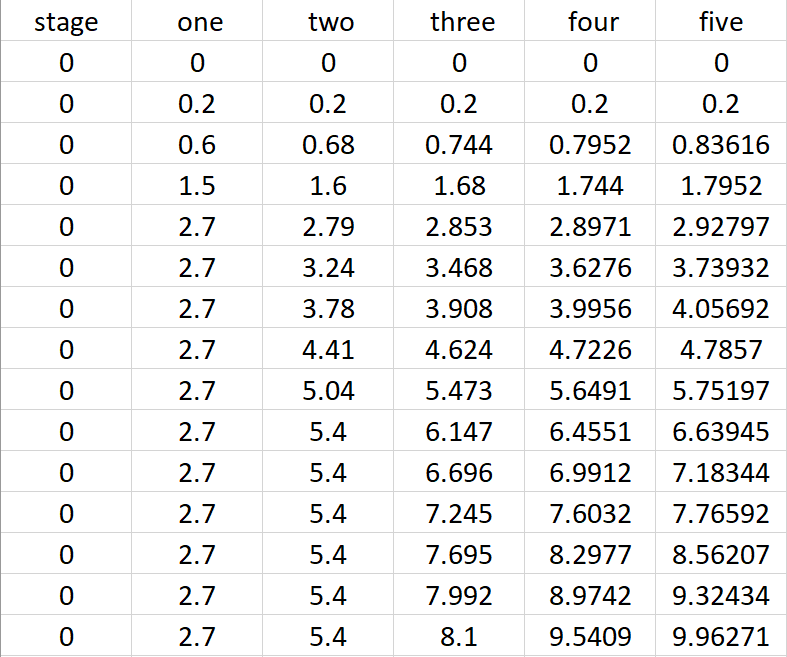
\includegraphics[width = 0.7\textwidth]{images/result1}
    \end{frame}

    % \begin{frame}{Extension}
    %
    % \end{frame}
